\appendix
\begin{center}
  \section{人员职责与分工}
\end{center}

\begin{itemize}
  \item 叶晓军:组长,主要负责项目人员组织、进度管理、系统业务逻辑设计
  \item 杨曦华:主要负责系统前端设计
  \item 柯毅豪:主要负责系统后台设计、系统部署
  \item 钟宇腾:主要负责系统架构设计、代码管理
  \item 系统测试与性能调优由全体成员共同完成。
\end{itemize}


\newpage

\begin{center}
  \section{系统开发日志}
\end{center}
\subsection{系统架构}
\begin{itemize}
  \item Django Web~框架(项目主页:https://www.djangoproject.com/)
  
  \CJKindent 本系统基于~django web~框架进行开发。~Django Web~框架是一个高级~Python\footnotemark[1] Web~框架,提供~ORM (~Object-relational mapper)~方法,可以完全使用~Python~来定义数据库的表及其元素,并封装了大量的数据库访问~API~,把数据库元素映射为~Python~内部类型,实现兼容多种数据库后台;提供~Template~系统,可以在~HTML~中嵌入~Python~代码便于服务器动态生成页面;提供缓存模块,提高服务器运行效率。
  
  \item Bootstrap前端框架与交互组件集(项目主页:http://twitter.github.com/bootstrap/)
  
  \CJKindent 本系统前端基于~Bootstrap~模板进行开发。~Bootstrap~是快速开发~Web~应用程序的前端工具包。它是一个~CSS~和~HTML~的集合,它使用了最新的浏览器技术,给~Web~开发提供了时尚的版式、表单、按钮、表格、网格系统等等。
\end{itemize}

\footnotetext[1]{Python~是一种面向对象的解析性编程语言、动态语言,支持命令式程序设计、面向对象程序设计、函数式编程、面向切面编程、泛型编程多种编程范式,具备垃圾回收功能,能够自动管理储存器使用。语言设计的哲学是“用一种方法,最好是只有一种方法来做一件事”,语法简洁少有岐义,代码可读性高。}

\subsection{代码托管与版本控制}
\begin{itemize}
  \item Git~版本控制系统
  
  \CJKindent Git~是一个由~Linus Benedict Torvalds~为了更好地管理~Linux~内核开发而创立的分布式版本控制/软件配置管理软件。与常用的版本控制工具~CVS、Subversion~等不同,它采用了分布式版本库的方式,不必服务器端软件支持,使源代码的发布和交流极其方便。~Git~的速度很快,这对于诸如~Linux kernel~这样的大项目来说自然很重要。~Git~最为出色的是它的合并跟踪(~merge tracing~)能力。
  
  \item GitHub
  
  \CJKindent GitHub~是一个用于使用~Git~版本控制系统的项目的基于互联网的存取服务,提供了像~feeds~,~followers~和显示开发者们怎样在他们的版本库的版本上工作的网络图表。根据在2009年的~Git~用户调查,~GitHub~是最流行的~Git~存取站点。
\end{itemize}

我们的项目托管于~GitHub~,项目地址为~https://github.com/zonyitoo/SYSUEduAdminSystem~,使用~Git~版本控制系统来进行版本控制和软件配置管理。

\begin{figure}[H]
   \centering 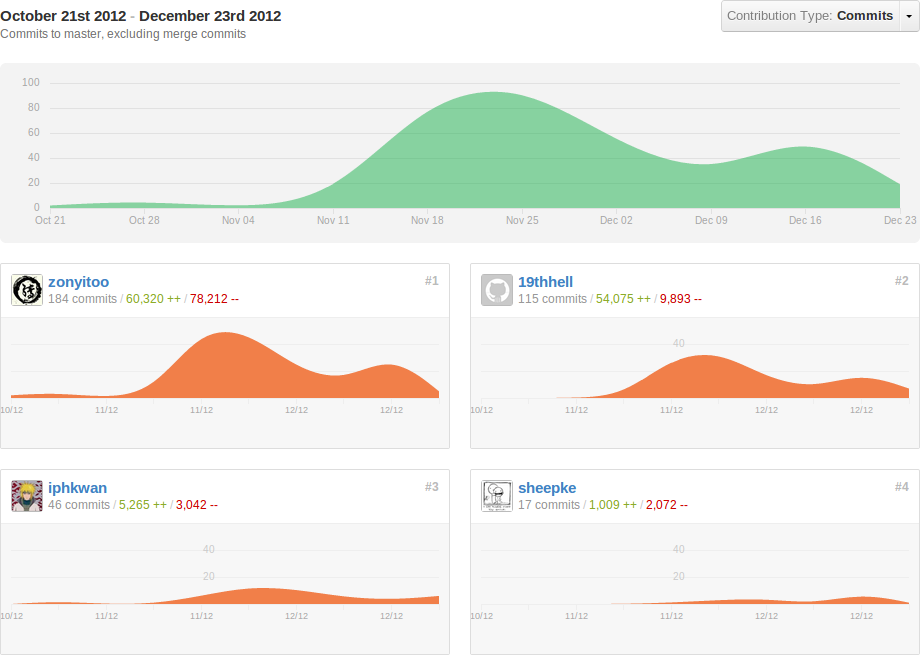
\includegraphics[width=\textwidth]{img/contrib.png}
   \caption{项目成员贡献及项目提交数与时间关系图}
\end{figure}

上图中,帐号与成员的对应关系为:钟宇腾(~zonyitoo~)、杨曦华(~19thhell~)、叶晓军(~iphkwan~)、柯毅豪(~sheepke~)。我们的项目从2012年10月21日开始编写,至2012年12月23日完成。在2012年11月20日前后进行基础框架搭建,并推出测试版,在2012年12月16日前后对于系统细节修补及加入新功能,推出第二个测试版。

钟宇腾(~zonyitoo~)是项目代码的管理员,主要负责项目文件树管理及架构设计,因此提交数(~Commits~)最多,增加了60320行代码,删除78212行代码;杨曦华(~19thhell~)是网页前端开发者,主要负责网页前端设计,有115次提交,增加了54075行代码,删除9893行代码;叶晓军(~iphkwan~)是组长,主要负责项目进度管理,有46次提交,增加5256行代码,删除3042行代码;柯毅豪(~sheepke~)是系统后台开发者,主要负责后台服务器响应代码编写及服务器维护及测试,有17次提交,增加1009行代码,删除2072行代码。

\begin{figure}[H]
   \centering 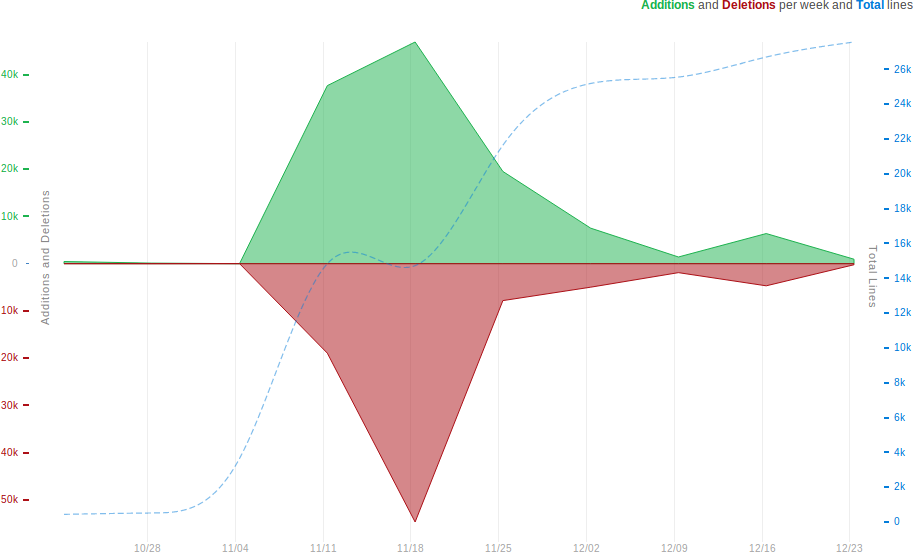
\includegraphics[width=\textwidth]{img/code_freq.png}
   \caption{项目代码变化图}
\end{figure}

图中蓝色虚线是代表代码行数的变化与时间的关系,2012年12月23日后代码行数超过了26万。绿色线的高度代表该时间段增加的代码行数,红色线的的高度代表该时间段被删除的代码行数,总体体现了代码增加的速度。
